% Chapter 5

\chapter{Results and discussion} % Main chapter title
\label{Chapter5} % For referencing the chapter elsewhere, use \ref{Chapter5} 
\section{Small Network solved by D-Wave CQM Sampler}
\subsection{D-Wave CQM ExactSolver()}
Since the problem we are tackling has just a few variables we can sample all the configuration space. For this task we use the \textit{CQM ExactSolver} class. One of the advantage of CQM is that it writes down if the solution is feasible, i.e.,  if that solution satisfy all the constraints of our problem. The solution of the problem is represented graphically in Figure\,\ref{fig: Green_final}.
\begin{figure}[H]
  \begin{center}
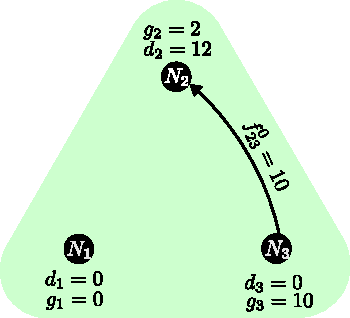
\includegraphics[width=0.4\textwidth]{Figures/Green_Final.pdf}
  \end{center}
  \caption{Graphical solution of three node problem.}
  \label{fig: Green_final}
\end{figure}
Notice that Table\,\ref{tab:SmallNetworkResults} represents only feasible solutions. They are sorted from lower energy to higher energy which means that the first row is the solution that minimizes the objective function by fulfilling the constraints, in this example the demand.
 \begin{table}[H]
\centering
\begin{tabular}{ |c|c|c|c|c|c|c|c| }
  \hline			
  $\mathbf{x_{12}}$ & $\mathbf{x_{13}}$ & $\mathbf{x_{23}}$ & $\mathbf{g_{1}}$ & $\mathbf{g_{2}}$ & $\mathbf{g_{3}}$ & \textbf{Prices} & \textbf{Feasible} \\
  \hline
    0 & 0 & 1 & 0 & 2 & 10 & 60 & True \\
  \hline
    0 & 0 & 1 & 0 & 3 & 9 & 63 & True \\
  \hline
    0 & 0 & 1 & 0 & 4 & 8 & 66 & True \\
  \hline
    0 & 0 & 1 & 0 & 6 & 7 & 69 & True \\
  \hline
\end{tabular}
\caption{D-Wave's feasible solutions to the TEP combinatorial optimization problem.}
\label{tab:SmallNetworkResults}
\end{table}
The optimal solution decides to build the most expensive transmission line, i.e., the one connecting nodes 2 and 3, and to use the maximum capacity of the cheapest generator, the one at node 3, see Table\,\ref{tab:SmallNetwork}.
%%%%%%%%%%%%%%%%%%%%%%%%%%%%%%%%%%%%%%%%%%%%%%%
\subsection{D-Wave LeapHybridCQMSampler()}
The implementation of TEP problems into D-Wave annealer requires of hybrid solvers due to the integers and real variables involved in the problem. For this reason, we implemented the  TEP problem from \textbf{INSERTAR RANGO DE ECUACIONES} in Python and use the D-Wave hybrid solver. As you may guess the results should be the same as the ones stated in the previous sections. However, in Table\,\ref{tab:SmallNetworkResultsHybrid} there are columns that did not appear before. The problem as stated here is general and takes into account every variable of TEP problems which do not happen with the formulation of last section.
 \begin{table}[H]
\centering
\begin{tabular}{ |c|c|c|c|c|c|c|c|c|c|c|c|c|c|c|c|c| }
  \hline			
  $\mathbf{x_{12}}$ & $\mathbf{x_{13}}$ & $\mathbf{x_{23}}$ & $\mathbf{f_{12}}$ & $\mathbf{f_{13}}$ & $\mathbf{f_{21}}$ & $\mathbf{f_{23}}$ & $\mathbf{f_{31}}$ & $\mathbf{f_{32}}$ &$\mathbf{g_{1}}$ & $\mathbf{g_{2}}$ & $\mathbf{g_{3}}$ & $\mathbf{r_{1}}$ & $\mathbf{r_{2}}$ & $\mathbf{r_{3}}$ &  \textbf{Prices} \\
  \hline
    0 & 0 & 1 & 0 & 0 & 0 & 10 & 0 & 0 & 0 & 2 & 10 & 0 & 0 & 0 & 60 \\
  \hline
  1 & 1 & 0 & 0 & 10 & 10 & 0 & 0 & 0 & 0 & 2 & 10 & 0 & 0 & 0 & 60 \\
  \hline
\end{tabular}
\caption{D-Wave's feasible solutions to the TEP combinatorial optimization problem.}
\label{tab:SmallNetworkResultsHybrid}
\end{table}
Notice that there are two solutions with the same cost. The first one has been shown in the previous section. However, the new solution produced by the hybrid solver build two lines whose accumulated cost is the same as the one connecting the node $3$ and the node $2$.
\begin{figure}[H]
  \begin{center}
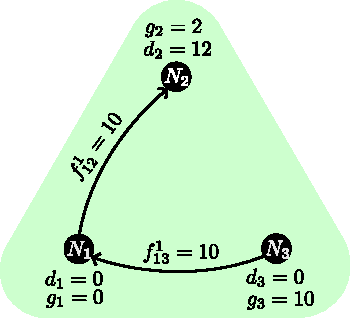
\includegraphics[width=0.4\textwidth]{Figures/3NodeGreenHybrid.pdf}
  \end{center}
  \caption{Graphical solution of three node problem.}
  \label{fig: Green_final_Hybrid}
\end{figure}

\begin{figure}[H]
  \begin{center}
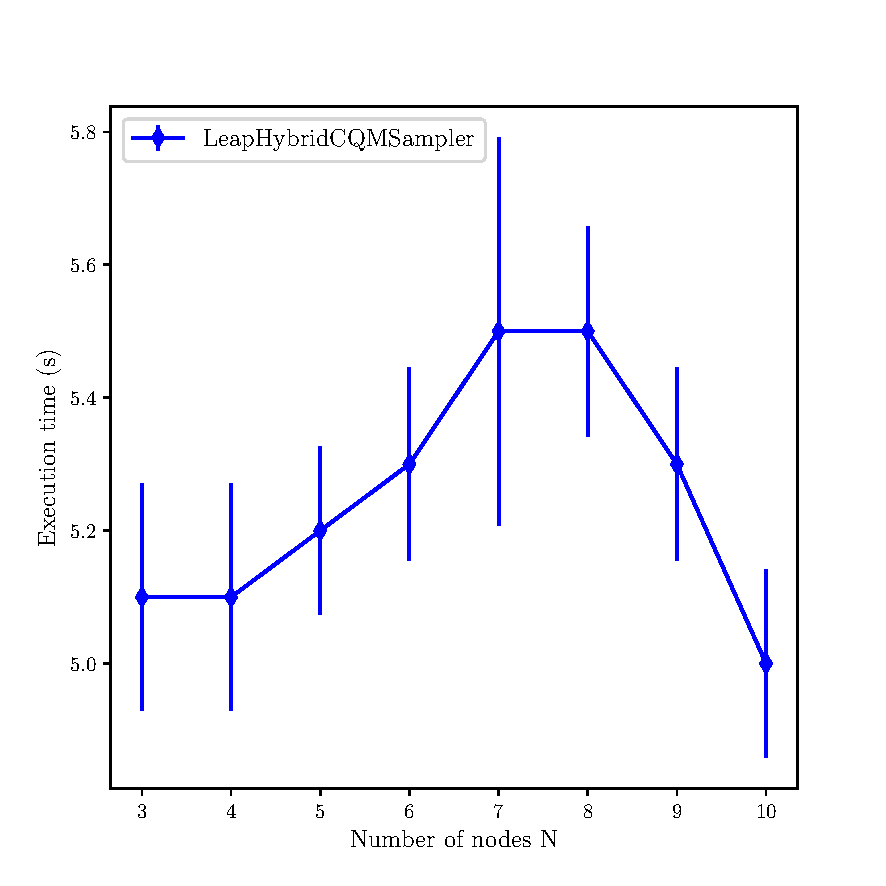
\includegraphics[width=0.8\textwidth]{Figures/ExecutionTimes.pdf}
  \end{center}
  \caption{Execution times for different test cases of small networks with D-Wave \textit{LeapHybridCQMSampler}.}
  \label{fig: ExecutionTimes}
\end{figure}

